\begin{frame}

    \frametitle{Température sans forçage}

    Sans forçage, la température varie linéairement pour une faible
    gradient. La variation devient non linéaire pour des gradients
    plus importants car, lorsque le gradient de température est augmenté,
    la conductivité thermique diminue.

    \setlength{\tabcolsep}{2pt}

    \begin{columns}

        \begin{column}{0.8\textwidth}
            \begin{figure}
                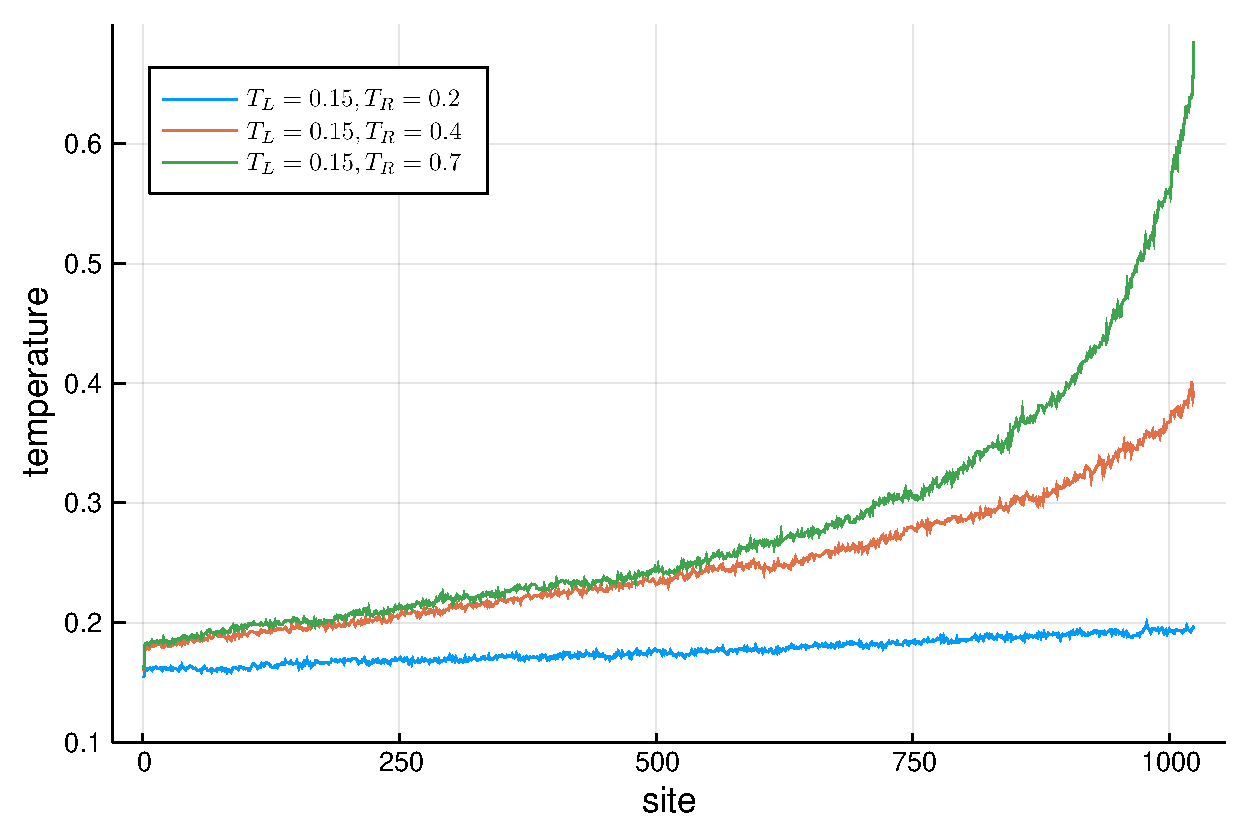
\includegraphics[scale=0.4]{plots/temperature_no_force.pdf}
            \end{figure}
        \end{column}

        \begin{column}{0.20\textwidth}
            \scriptsize
            Rotors : 1024
            Sans forçage
        \end{column}

    \end{columns}

\end{frame}

\begin{frame}

    \frametitle{Température}

    La température est maximum vers le milieu de la chaîne, et
    la position de ce maximum dépend des valeurs des thermostats.

    \begin{columns}

        \begin{column}{0.8\textwidth}
            \begin{figure}
                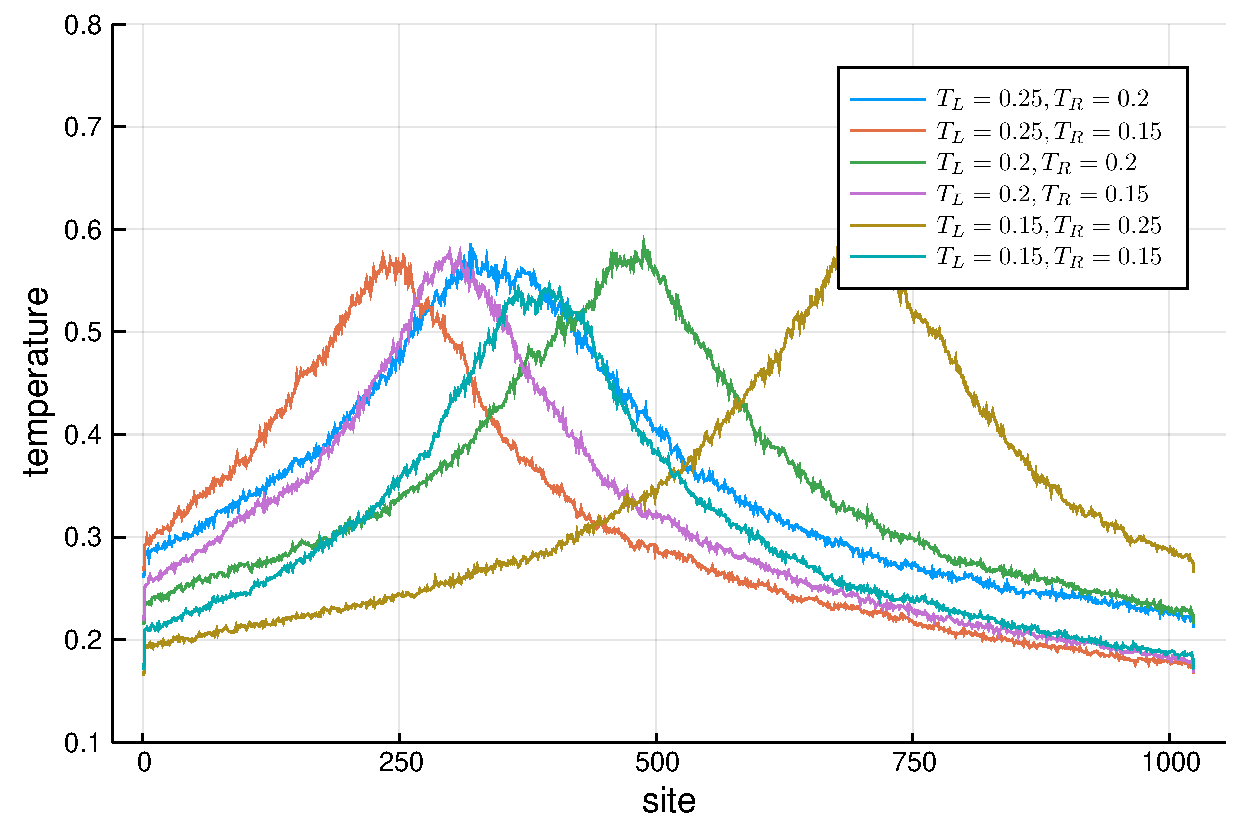
\includegraphics[scale=0.4]{plots/temperature.pdf}
            \end{figure}
        \end{column}

        \begin{column}{0.2\textwidth}
            \scriptsize
            Rotors : 1024
            Forçage : 1.6
        \end{column}

    \end{columns}

\end{frame}

\begin{frame}

    \frametitle{Impulsion Moyenne}

    Le profil de l'impulsion moyenne n'est pas linéaire, et la
    position de sa dérivée maximale coïncide avec la position de
    la température maximale.

    \begin{columns}

        \begin{column}{0.8\textwidth}
            \begin{figure}
                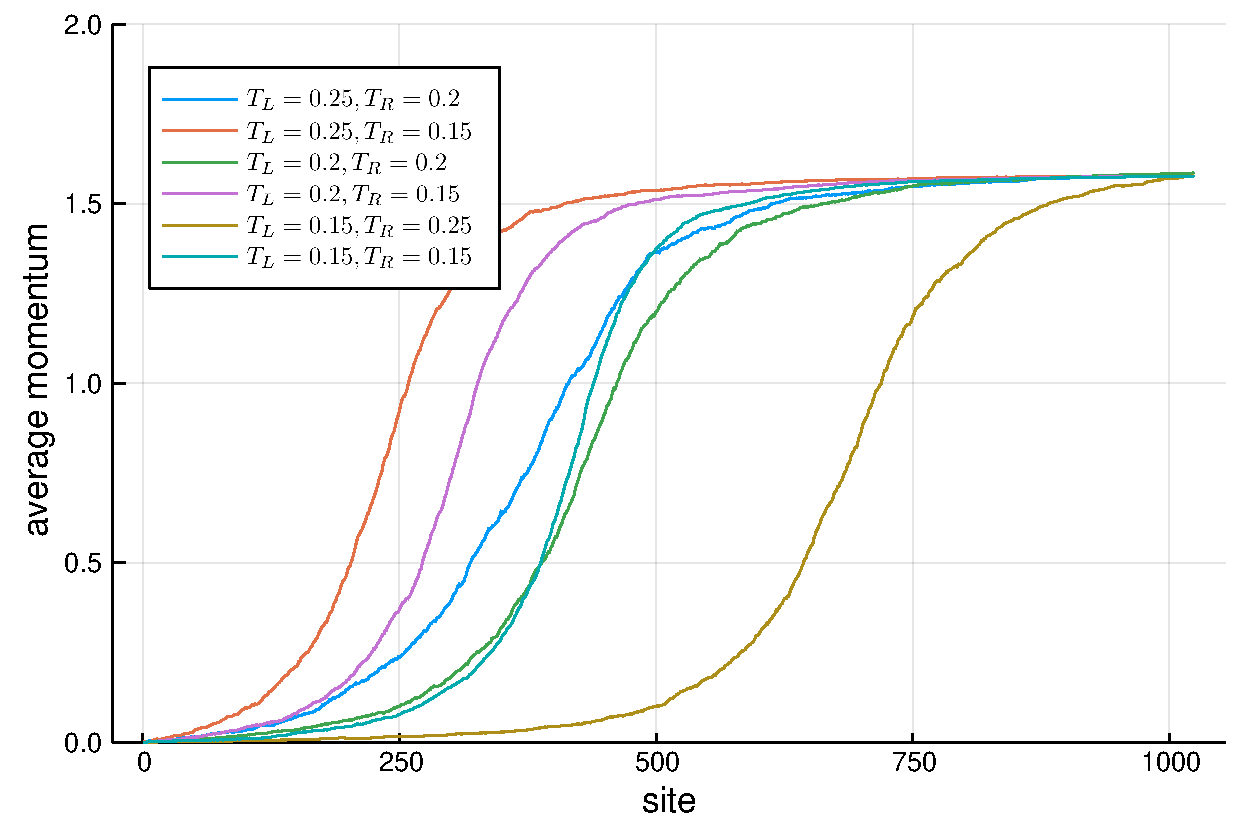
\includegraphics[scale=0.4]{plots/average_momentum.pdf}
            \end{figure}
        \end{column}

        \begin{column}{0.2\textwidth}
            \scriptsize
            Rotors : 1024
            Forçage : 1.6
        \end{column}

    \end{columns}

\end{frame}

\begin{frame}

    \frametitle{Impulsion Moyenne}

    L'impulsion moyenne pour des chaînes de longueurs différentes
    sur la même échelle.

    \begin{columns}

        \begin{column}{0.8\textwidth}
            \begin{figure}
                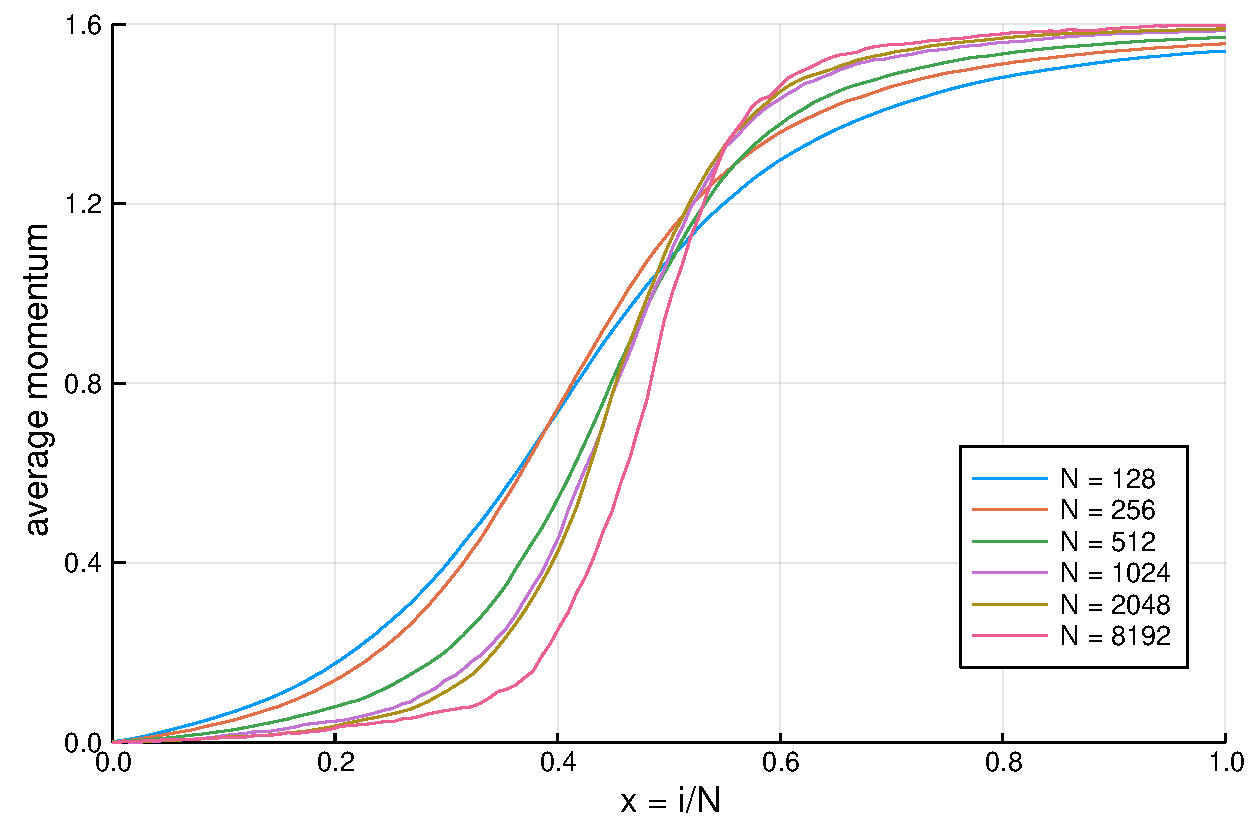
\includegraphics[scale=0.4]{plots/average_momentum_scaled.pdf}
            \end{figure}
        \end{column}

        \begin{column}{0.2\textwidth}
            \scriptsize
            Forçage : 1.6 \\
            $T_L$ : 0.2 \\
            $T_R$ : 0.2
        \end{column}

    \end{columns}

\end{frame}

\begin{frame}

    \frametitle{Température cinétique et potentielle}

    Pour les chaînes les plus longues on a l'accord entre la
    température cinétique (lignes solides) et la température
    potentielle.

    \begin{columns}

        \begin{column}{0.8\textwidth}
            \begin{figure}
                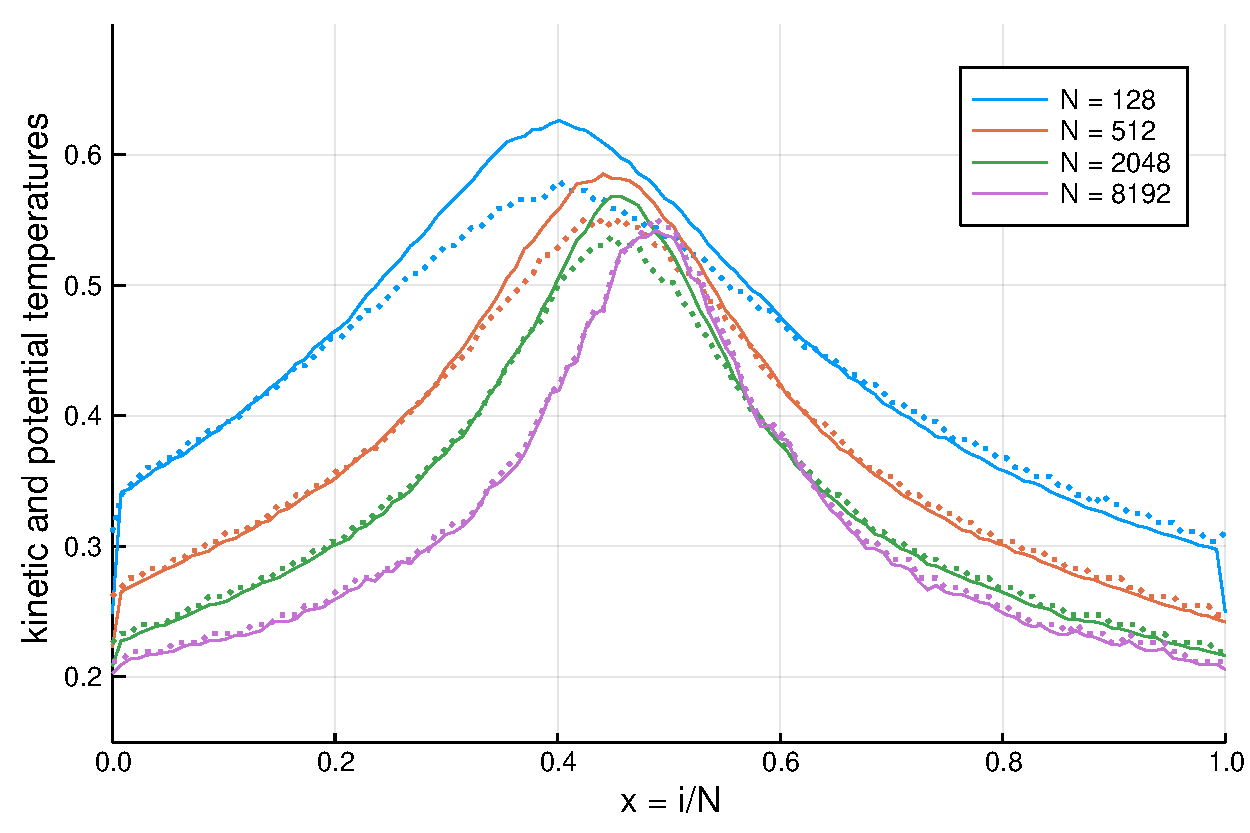
\includegraphics[scale=0.4]{plots/temperature_scaled.pdf}
            \end{figure}
        \end{column}

        \begin{column}{0.2\textwidth}
            \scriptsize
            Cinétique : \\
            ligne solide \\
            \vspace{3mm}
            Potentielle : \\
            ligne pointillée

        \end{column}

    \end{columns}

\end{frame}

\begin{frame}

    \frametitle{Distribution de l'impulsion}

    Distribution empirique de l'impulsion du rotor le plus chaud,
    et la distribution de Gibbs :
    $Z_\text{kin}^{-1} \exp[-(p - \overline p_i)^2 / (2T_i)]$,
    où $i$ est l'index du rotor le plus chaud et
    $Z_\text{kin} = \sqrt{2 \pi T_i}$.

    \begin{columns}

        \begin{column}{0.8\textwidth}
            \begin{figure}
                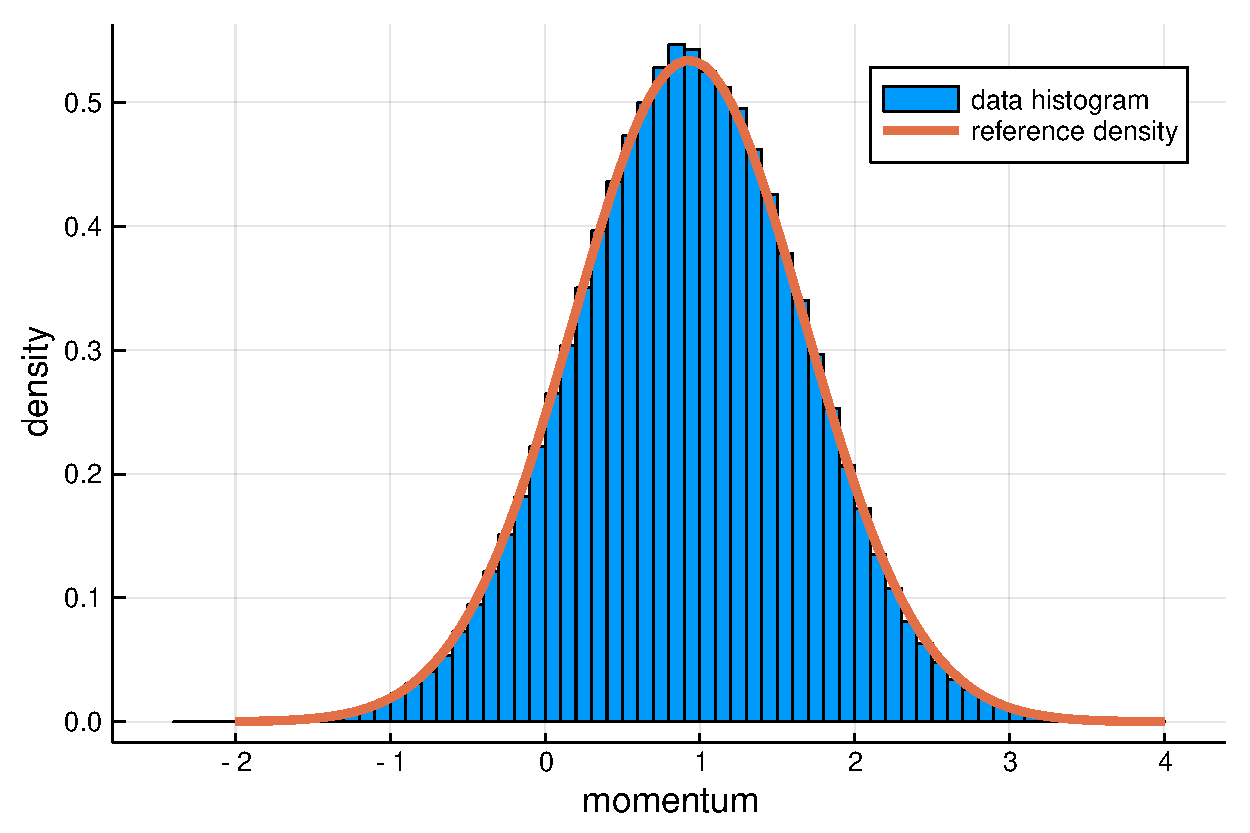
\includegraphics[scale=0.4]{plots/gibbs_momentum.pdf}
            \end{figure}
        \end{column}

        \begin{column}{0.2\textwidth}
            \scriptsize
            Rotors : 1024
            Forçage : 1.6
            $T_L = T_R = 0.2$
        \end{column}

    \end{columns}

\end{frame}

\begin{frame}

    \frametitle{Distribution de la distance}

    Distribution empirique de la distance du rotor le plus chaud
    (à son voisin), et la distribution de Gibbs :
    $Z_\text{pot}^{-1} \exp[-V(r) / T_i]$,
    où $i$ est l'index du rotor le plus chaud.
%    et $Z_\text{pot}$ est calculé.

    \begin{columns}

        \begin{column}{0.8\textwidth}
            \begin{figure}
                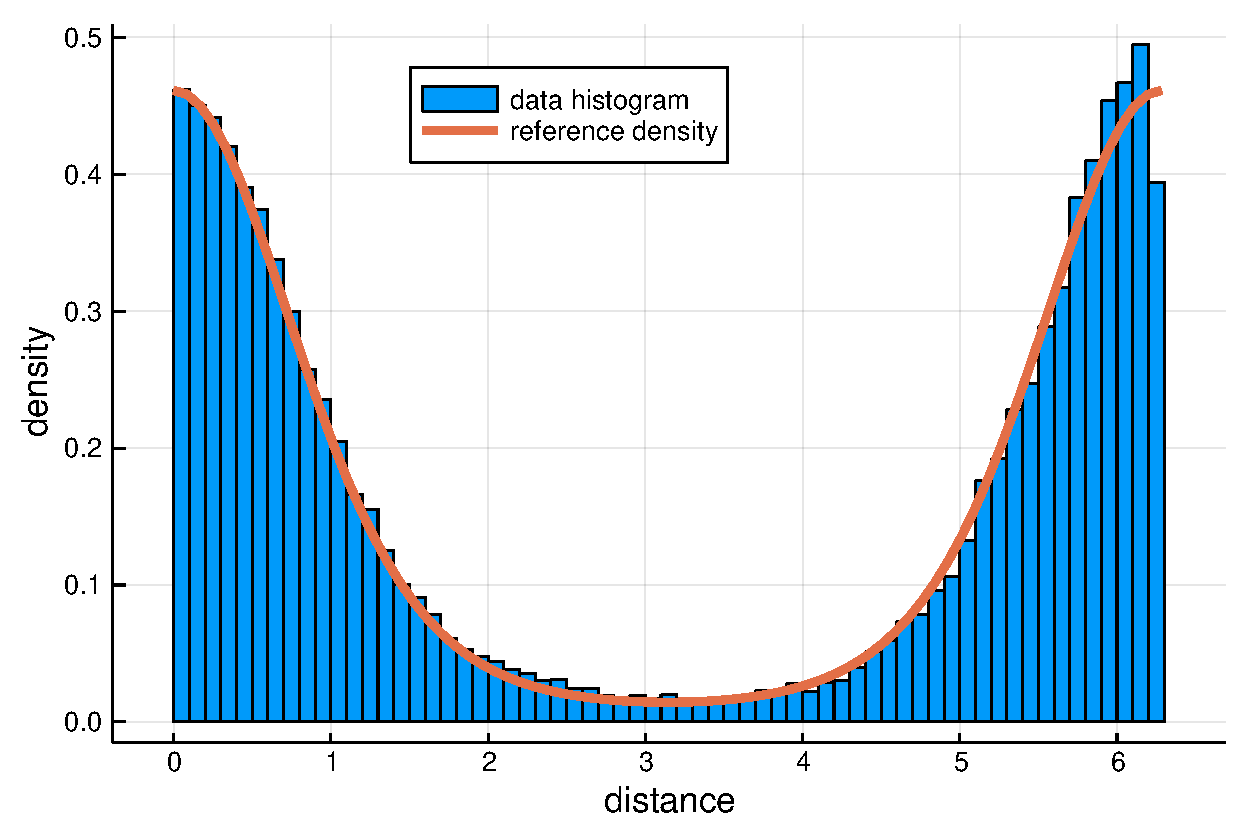
\includegraphics[scale=0.4]{plots/gibbs_distance.pdf}
            \end{figure}
        \end{column}

        \begin{column}{0.2\textwidth}
            \scriptsize
            Rotors : 1024
            Forçage : 1.6
            $T_L = T_R = 0.2$
        \end{column}

    \end{columns}

\end{frame}

\begin{frame}

    \frametitle{Indépendance des impulsions et distances}

    Décroissance de l'erreur par rapport au nombre d'échantillons
    entre la distribution jointe et le produit tensoriel des
    impulsions et des distances.
    %
    $\delta_n = \int_{[0,2\pi] \times \mathbb{R}} |\psi^n(r,p)
    - \overline \psi^n(r) \overline \psi^n(p)]| dr dp.$

    \begin{columns}

        \begin{column}{0.8\textwidth}
            \begin{figure}
                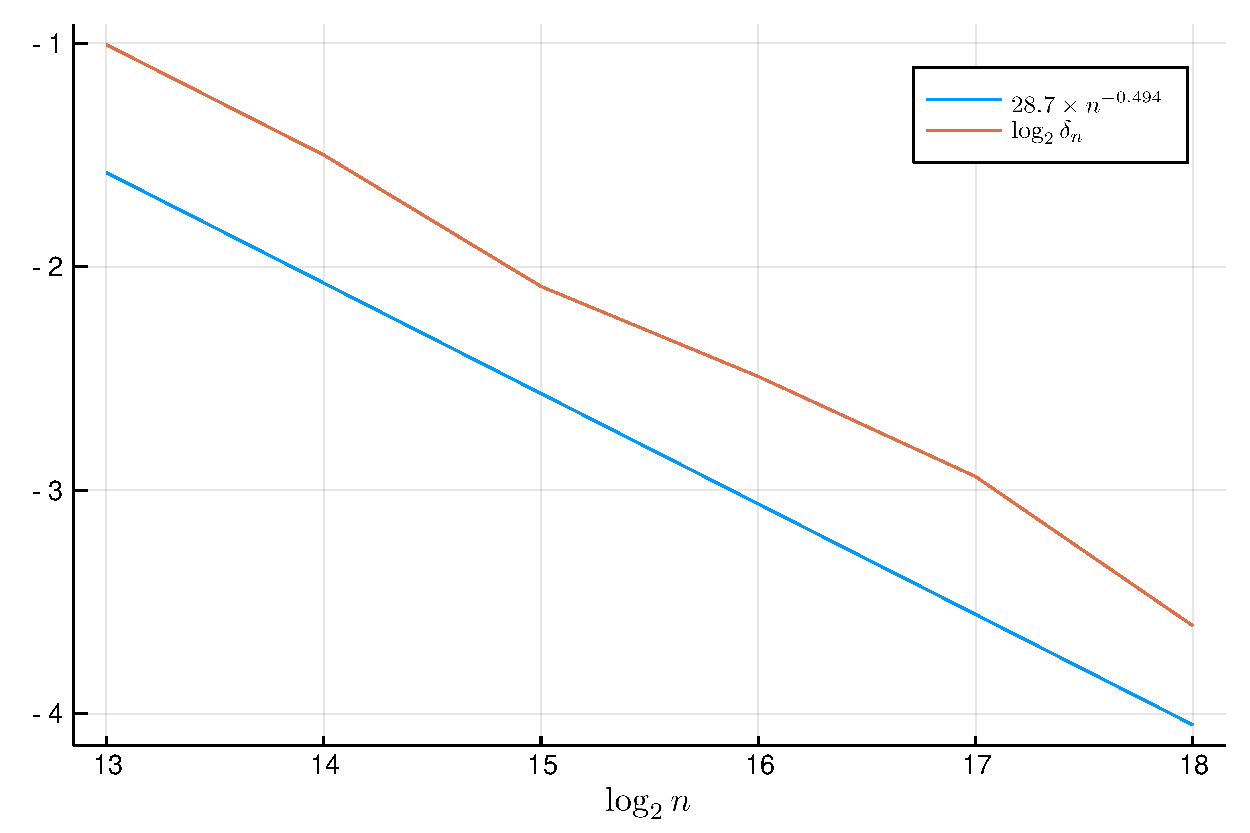
\includegraphics[scale=0.4]{plots/distribution_error.pdf}
            \end{figure}
        \end{column}

        \begin{column}{0.2\textwidth}
            \scriptsize
            Rotors : 1024
            Forçage : 1.6
            $T_L = T_R = 0.2$

            \vspace{2.0mm}

            Décroissement :
            $\delta_n \approx 13 \times n^{-0.491}$

        \end{column}

    \end{columns}

\end{frame}

\begin{frame}

    \frametitle{Flux d'énergie normal}

    Le flux d'énergie par rapport au forçage pour des chaînes de longueurs
    différentes. La température à droite est 0.15. La couleur des courbes
    indique la température á gauche (0.15, 0.2, et 0.25).

    \begin{columns}

        \begin{column}{0.8\textwidth}
            \begin{figure}
                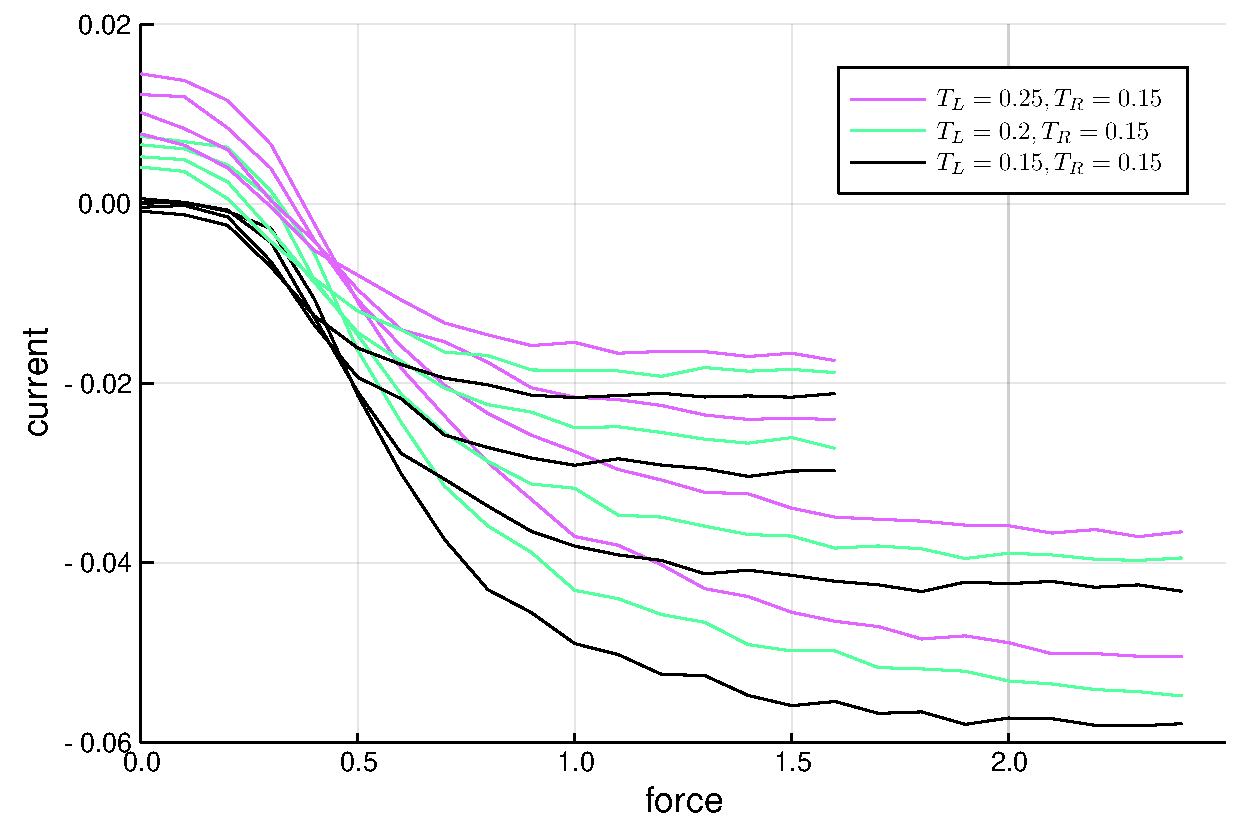
\includegraphics[scale=0.4]{plots/energy_current_normal.pdf}
            \end{figure}
        \end{column}

        \begin{column}{0.2\textwidth}

            \scriptsize

            \vspace{18.0mm}
            N = 1024

            \vspace{3.0mm}
            N = 512

            \vspace{4.0mm}
            N = 256

            \vspace{5.0mm}
            N = 128

        \end{column}

    \end{columns}

\end{frame}

\begin{frame}

    \frametitle{Flux d'énergie étrange}

    Ici, la réduction de la température à droite suscite une
    \alert{augmentation} du courant vers la gauche. Une explication est
    que la réduction de température augmente la conductivité, et donc
    le forçage a davantage d'influence sur le système.

    \begin{columns}

        \begin{column}{0.8\textwidth}
            \begin{figure}
                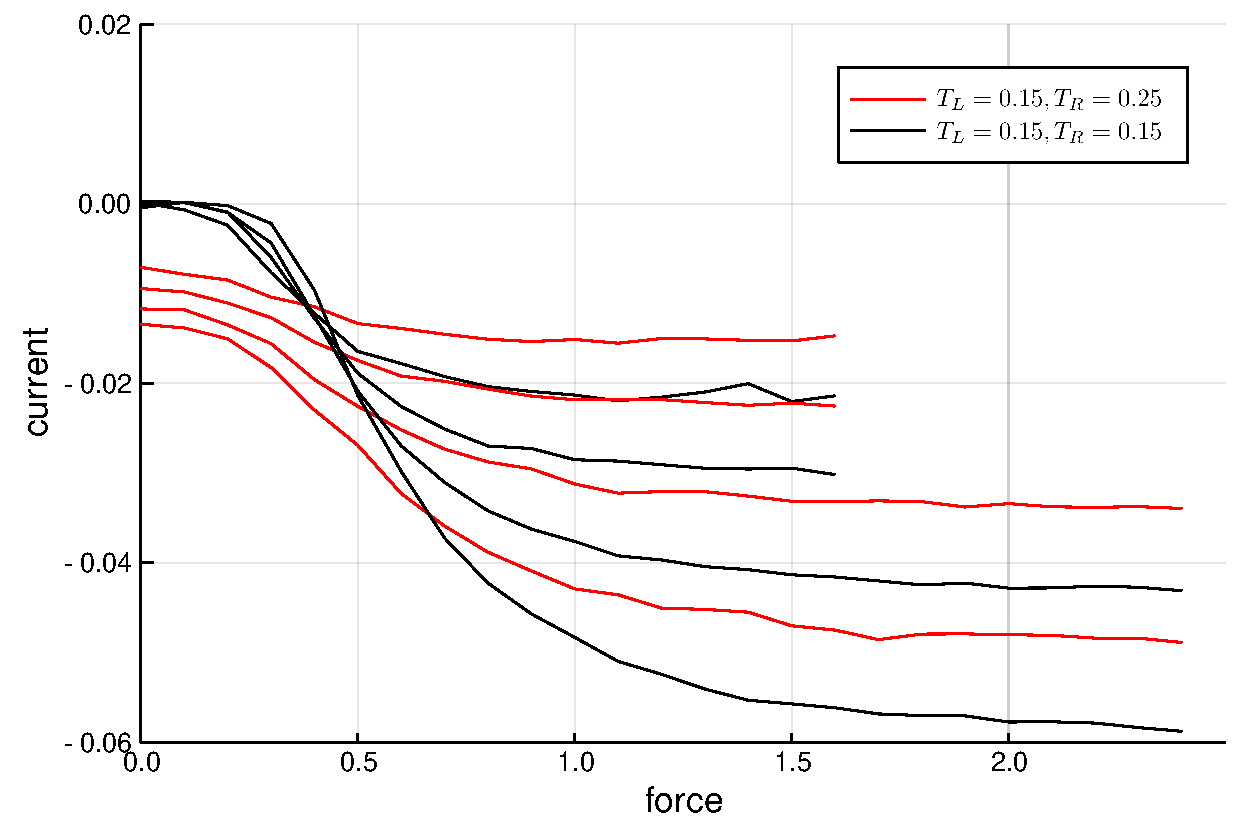
\includegraphics[scale=0.4]{plots/energy_current_strange.pdf}
            \end{figure}
        \end{column}

        \begin{column}{0.2\textwidth}

            \scriptsize

            \vspace{15.0mm}
            N = 1024

            \vspace{3.0mm}
            N = 512

            \vspace{4.0mm}
            N = 256

            \vspace{5.0mm}
            N = 128

        \end{column}

    \end{columns}

\end{frame}
